\documentclass{boi2014-dk}

\usepackage{enumitem}

\renewcommand{\DayNum}{2}
\renewcommand{\TaskCode}{portals}
\renewcommand{\TaskName}{Portals}
\renewcommand{\TaskVersion}{1.1}

\newcommand{\constant}[1]{{\tt #1}}

\begin{document}
    \begin{wrapfigure}[4]{r}{4cm}
        \vspace{-24pt}
		\includegraphics[width=4cm]{\TaskCode.jpeg}
	\end{wrapfigure}

    Der er en kage placeret i en labyrint, og du er desperat for at spise
    den. Du har et kort over labyrinten, som er et gitter med $R$ rækker og $C$
    kolonner. Hver celle i gitteret indeholder et af følgende tegn:
    \begin{description}[itemindent=1pt]
    	\item[\constant{\#}] (hashtag) er en murblok,
        \item[\constant{.}] (punktum) er en åben plads,
        \item[\constant{S}] (stort s) er en åben plads som er din
            nuværende position,
        \item[\constant{C}] (stort c) er en åben plads hvor kagen er.
    \end{description}

    Du må kun gå på de åbne pladser, og du kan kun bevæge dig fra en åben plads
    til en anden, hvis de deler en side. Derudover er det rektangulære område
    givet på kortet fuldstændigt omgivet af samme slags murblokke.

    For at kunne nå til kagen hurtigere har du anskaffet et portal-gevær
    fra Aperture Science\texttrademark{}, der fungerer som følger.
    Til et hvert tidspunkt kan den skyde en portal i en af de fire rætninget
    \em{op}, \em{venstre}, \em{ned} og \em{højre}. Når en portal bliver skudt i
    en retning, vil den flyve i den rætning ind til den rammer den første
    murblok. Når det sker, vil der komme portal på den side af murblokken,
    der vender mod dig.

    Der kan højest være to portaler på et hvilket som helst tidspunkt. Hvis der
    allerede er to portaler i labyrinten, så vil en af dem (valgt af dig) blive
    fjernet samme tid som du bruger portal-geværet igen. Hvis du skyder en
    portal på en eksisterende portal vil den blive erstattet
    (der kan højest være en portal pr.~side af en murblok). Bemærk, at der
    kan være portaler på forskellige sider af den samme murblok.

    Så snart der er to portaler på kortet kan du bruge dem til at teleportere
    dig. Når du står ved siden af en af portalerne kan du gå ind i den og komme
    ud af den anden. At gøre dette tager lige så lang tid som at gå mellem to
    tilstødende pladser.

    Du kan antage, at det ikke tager tid at skyde med portal-geværet og at
    bevæge sig mellem to tilstødende pladser eller at teleportere sig med
    portaler tager én tidsenhed.

    \Task
    Givet et kort over labyrinten sammen med din startposition og kagens
    position, beregn det mindste antal tidsenheder du skal bruge for at nå til
    kagen.

    \Input
    Den første linje af input indeholder to heltal: Antallet af rækker på
    kortet, $R$, og antallet af kolonner $C$. De næste $R$ linjer beskriver
    kortet. Hver linje indeholder $C$ tegn: \constant{\#},
    \constant{.}, \constant{S} or \constant{C} (hvis betydning er som beskrevet
    ovenfor).

    Det er garanteret, at \constant{S} og \constant{C} hver optræder præcis en
    gang på kortet.

    \Output
    Outputtet skal indeholde et enkelt heltal -- det mindste antal tidsenheder
    der skal bruges for at nå til kagen fra startpositionen.

    Du kan antage, at det er muligt at nå til kagen fra din startposition.

    \Example
    \example
    {
        4 4\newline
        .\#.C\newline
        .\#.\#\newline
        ....\newline
        S...
    }
    {
        4
    }
    {
        En sekvens af træk, der når kagen hurtigst er som følger: 1) gå til
        højre, 2) gå til højre, skyd en portal op og en ned, 3) gå igennem
        bundportalen -- Du vil nu være på position ($række = 0, kolonne = 2$),
        4) gå til højre og nå kagen.

        \begin{center}
            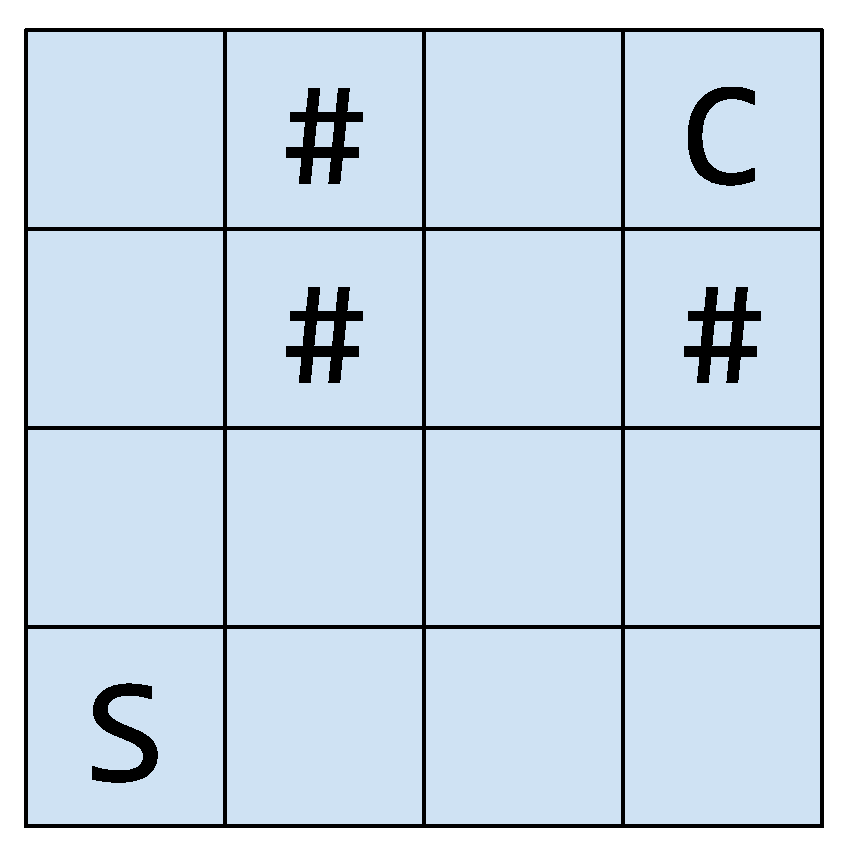
\includegraphics[width=4cm]{portals-example}
        \end{center}
    }

    \Scoring

    \begin{description}[leftmargin=0pt]
        \item[Delopgave 1 (? point):] $1 \le R \le 10, 1 \le C \le 10$.
        \item[Delopgave 2 (? point):] $1 \le R \le 50, 1 \le C \le 50$.
        \item[Delopgave 3 (? point):] $1 \le R \le 200, 1 \le C \le 200$.
            Enhver åben plads har mindst en tilstødende mur.
        \item[Delopgave 4 (? point):] $1 \le R \le 200, 1 \le C \le 200$.
        \item[Delopgave 5 (? point):] $1 \le R \le 1000, 1 \le C \le 1000$.
    \end{description}

    \Constraints

    \begin{description}
        \item[Tidsbegrænsning:] 1 s.
        \item[Hukommelsesbegrænsning:] 256 MB.
    \end{description}
\end{document}
